\chapter{Liquid Dynamics}

The dynamics of a molecular system is characterised by two main elements, the diffusion of the particles through the liquid and the rotational motion of those particles. Understanding these properties of the liquid provide the basis for further study giving estimates of the timescales that events are likely to occur at. It also provides important information about the range of temperatures at which the particular system can be studied. The molecules that we have chosen for study in this thesis are shown in \textfigref{my mols}. These three molecules were chosen as they represent a wide range of concavity, from the small concavity in the \sone molecule through to the large concavity in the \tri molecule. This difference in concavity if expected to give rise to differing dynamical behaviour, particularly the fragility.

\begin{figure}
    \centering
    \captionsetup{justification=centering}
    \begin{subfigure}[t]{0.3\textwidth}
        \includegraphics[width=\linewidth]{{{Snowman-0.637556-1.0}}}
        \caption{\dimer{0.637556}{1.0} \\\sone}
        \label{fig:sone}
    \end{subfigure}
    \begin{subfigure}[t]{0.3\textwidth}
        \includegraphics[width=\linewidth]{{{Snowman-0.637556-1.637556}}}
        \caption{\dimer{0.637556}{1.637556} \\\scon}
        \label{fig:scon}
    \end{subfigure}
    \begin{subfigure}[t]{0.3\textwidth}
        \includegraphics[width=\linewidth]{{{Trimer-0.637556-1.00-120}}}
        \caption{\trimer{0.637556}{1.0}{120} \\\tri}
        \label{fig:tri}
    \end{subfigure}
    \caption[Molecules chosen for further study]{The molecules chosen for study in this thesis in order of the size of the concavity. The \sone with the smallest concavity, \scon with the smaller disc contacting and \tri with a concavity larger than the large disc.}
    \label{fig:my mols}
\end{figure}

\section{Dynamics of \sone}

\begin{figure}
    \begin{subfigure}[t]{0.5\linewidth}
        \includegraphics[width=\textwidth]{{{Snowman-0.637556-1.0-msd}}}
        \caption{MSD}
        \label{fig:snowman 0.637556 1.0 msd}
    \end{subfigure}
    \begin{subfigure}[t]{0.5\linewidth}
        \includegraphics[width=\textwidth]{{{Snowman-0.637556-1.0-P1(t)}}}
        \caption{R1}
        \label{fig:snowman 0.637556 1.0 r1}
    \end{subfigure}
    \begin{subfigure}{0.5\textwidth}
        \includegraphics[width=\textwidth]{{{Snowman-0.637556-1.0-F}}}
        \caption{Structure Function}
        \label{fig:snowman 0.637556 1.0 structure}
    \end{subfigure}
    \begin{subfigure}{0.5\textwidth}
        \includegraphics[width=\textwidth]{{{Snowman-0.637556-1.0-P2(t)}}}
        \caption{R2}
        \label{fig:snowman 0.637556 1.0 r2}
    \end{subfigure}
    \caption{The main dynamical features of the \sone molecule.}
    \label{fig:snowman 0.637556 1.0}
\end{figure}

With the main dynamical quantities of interest being the translation of the center of mass (COM) and the rotation it makes sense to represent the particles as the center of mass and an orientation vector. This method is independent of the number of particles making analysis simple, allowing us to find the Mean Squared Displacement (MSD) a measure of the translational motion which when differentiated can be used to find the diffusion constant. The MSD for \sone over a range of temperatures is shown in \textfigref{snowman 0.637556 1.0 msd}. The initial region up to approximately $10^1$ timesteps is the ballistic region where the particles are yet to collide with each other. At higher temperatures the transition from the ballistic to the diffusive regime is seamless. The diffusive regime is defined by a MSD that increases as a linear function of $t$, indicated by the grey line on the plot. At lower temperatures like 0.90 (shown in red) there is a distinct levelling off of the MSD between the ballistic and diffusive regimes. This region of slow diffusion is where there are only a small number of particles that have escaped their local minima, they still have the same neighbours that they started with and are vibrating within the bounds of those neighbours.

The orientation of the molecule allows us to define a rotational relaxation, a measure of the type of rotational motions that take place. There are two rotational relaxations we are concerned with, R1 is a measure of the small angular steps that take place while R2 is concerned with orientational flips that take place. Both of these relaxations are used to give us information about the type of relaxations that take place, large differences between R1 and R2 would be indicative of a process dominated by large jumps in the orientation. Instead we have observed very similar behaviour between R1~\figref{snowman 0.637556 1.0 r1} and R2~\figref{snowman 0.637556 1.0 r2}. Again like the MSD we see the stagnation of the relaxation at low temperatures.

Another dynamical quantity that we were interested in is the Structure Function $F(t)$. This is a deviation from the COM and orientation that we have been using to define previous dynamical quantities. The Structure function instead uses the position of each individual particle. The approach is used as it allows us to combine both the rotations and translations of a molecule into a single function. The Structure function is given by
\begin{align}
    F(t) = \begin{cases}
        \quad0 &\text{if } \Delta \vect x > 0.3 \\
        \quad1 &\text{if } \Delta \vect x \leq 0.3
    \end{cases}
\end{align}
where $\Delta \vect x$ is the distance of each particle from its initial position. The value of $0.3$ was chosen to be small enough to be able to observe the combination of translational and rotational relaxations. The Structure function for \sone is shown in \textfigref{snowman 0.637556 1.0 structure} and shows some interesting characteristics. The initial region between \num{e0} and \num{e1} timesteps is flat as the particles have not had enough time to move \si{0.3} units in distance. The sharp dropoff, characteristic of the binary function matches closely with the time that the MSD transitions from the ballistic regime indicative of the molecules escaping their local environment. The other interesting feature is the increase in the Structure function for low temperatures at \num{e4}. This can be explained by the molecular vibrations or rotations of molecules within their initial local environment. Particles will move outside the cutoff distance as part of a vibration and return to their initial positions resulting in the periodicity of the vibrations.

All the properties so far have been investigating the bulk properties of the molecules, however in the highly supercooled region in which we are interested in, the dynamics of the system are often heterogeneous, there are spatially separated regions of highly mobile particles and regions of slow moving particles. \textfigref{snowman 0.637556 1.0 moved} shows that \sone exhibits areas of both dynamic and rotational heterogeneity. There is a strong correlation between the regions of dynamic and rotational motion, however it is not a direct correlation, there are both particles that have moved a long way with a small rotation and particles that have moved a very short distance with a large rotation.

The visual inspection of these homogeneities tells us that they exist but makes it difficult to make comparisons. To do this we can use a variety of functions designed to compare dynamic homogeneities. These functions are based on finding the variance of dynamic variables over the frame.

\begin{figure}
    \centering
    \includegraphics[width=0.75\textwidth]{{{Snowman-0.637556-1.0-moved}}}
    \caption{Movement of particles within a frame. This shows the net motions of all \sone molecules over a simulation run. The motion of the centers of mass are displayed by the vectors, directly representing the motion that took place. The magnitude of the rotation is given by the intensity of the green circles.}
    \label{fig:snowman 0.637556 1.0 moved}
\end{figure}

The first of these measures in the nongaussian parameter $\alpha(t)$ which is a measure of the deviation of the MSD from a gaussian distribution, what would be expected if the motion for all particles was truly randomly distributed~\figref{snowman 0.637556 1.0 alpha}.

\begin{figure}
    \centering
    \includegraphics[width=0.5\linewidth]{{{Snowman-0.637556-1.0-alpha}}}
    \caption{Nongaussian function}
    \label{fig:snowman 0.637556 1.0 alpha}
\end{figure}

Another of these gives a value for a characteristic length scale and the relaxation time of the dynamic inhomogeneities, the $\chi_4(t)$ function~\figref{snowman 0.637556 1.0 chi4}. This is given by the variance of the structure function at each time point. 

\begin{figure}
    \centering
    \includegraphics[width=0.5\linewidth]{{{Snowman-0.637556-1.0-chi}}}
    \caption{$\chi_4(t)$}
    \label{fig:snowman 0.637556 1.0 chi4}
\end{figure}

All these same functions can also be applied to the other systems we are studying

\section{Dynamics of \scon}

\begin{figure}
    \begin{subfigure}{0.5\linewidth}
        \includegraphics[width=\textwidth]{{{Snowman-0.637556-1.637556-msd}}}
        \caption{MSD}
        \label{fig:snowman 0.637556 1.637556 msd}
    \end{subfigure}
    \begin{subfigure}{0.5\linewidth}
        \includegraphics[width=\textwidth]{{{Snowman-0.637556-1.637556-P1(t)}}}
        \caption{R1}
        \label{fig:snowman 0.637556 1.637556 r1}
    \end{subfigure}
    \begin{subfigure}{0.5\textwidth}
        \includegraphics[width=\textwidth]{{{Snowman-0.637556-1.637556-F}}}
        \caption{structure function}
        \label{fig:snowman 0.637556 1.637556 structure}
    \end{subfigure}
    \begin{subfigure}{0.5\textwidth}
        \includegraphics[width=\textwidth]{{{Snowman-0.637556-1.637556-P2(t)}}}
        \caption{r2}
        \label{fig:snowman 0.637556 1.637556 r2}
    \end{subfigure}
    \caption{Snowman 0.637556 1.637556}
    \label{snowman 0.637556 1.637556}
\end{figure}

\begin{figure}
    \centering
    \includegraphics[width=0.5\linewidth]{{{Snowman-0.637556-1.637556-alpha}}}
    \caption{Nongaussian function}
    \label{fig:snowman 0.637556 1.637556 alpha}
\end{figure}

\begin{figure}
    \centering
    \includegraphics[width=0.5\linewidth]{{{Snowman-0.637556-1.637556-chi}}}
    \caption{$\chi_4(t)$}
    \label{fig:snowman 0.637556 1.637556 chi4}
\end{figure}

\section{Dynamics of \tri}

\begin{figure}
    \begin{subfigure}{0.5\linewidth}
        \includegraphics[width=\textwidth]{{{Trimer-0.637556-1.00-120-msd}}}
        \caption{MSD}
        \label{fig:trimer 0.637556 1.0 120 msd}
    \end{subfigure}
    \begin{subfigure}{0.5\linewidth}
        \includegraphics[width=\textwidth]{{{Trimer-0.637556-1.00-120-P1(t)}}}
        \caption{R1}
        \label{fig:trimer 0.637556 1.0 120 r1}
    \end{subfigure}
    \begin{subfigure}{0.5\textwidth}
        \includegraphics[width=\textwidth]{{{Trimer-0.637556-1.00-120-F}}}
        \caption{structure function}
        \label{fig:trimer 0.637556 1.0 120 structure}
    \end{subfigure}
    \begin{subfigure}{0.5\textwidth}
        \includegraphics[width=\textwidth]{{{Trimer-0.637556-1.00-120-P2(t)}}}
        \caption{r2}
        \label{fig:trimer 0.637556 1.0 120 r2}
    \end{subfigure}
    \caption{Trimer 0.637556 1.0 120}
    \label{fig:trimer 0.637556 1.0 120}
\end{figure}

\begin{figure}
    \centering
    \includegraphics[width=0.5\linewidth]{{{Trimer-0.637556-1.00-120-alpha}}}
    \caption{Nongaussian function}
    \label{fig:trimer 0.637556 1.0 120 alpha}
\end{figure}

\begin{figure}
    \centering
    \includegraphics[width=0.5\linewidth]{{{Trimer-0.637556-1.00-120-chi}}}
    \caption{$\chi_4(t)$}
    \label{fig:trimer 0.637556 1.0 120 chi4}
\end{figure}


\section{Comparison}

By themselves these functions don't allow easy comparison between different molecules. For this we can represent these functions as a single value, the MSD can be sufficiently represented as the diffusion constant, the constant for the linear region. For the structure function and the rotation functions we can define a relaxation time, the time it takes for the functions to reach a value of $1/\e$. This value is chosen as the relaxation is typically exponential, so this is representative of half the time to zero.\tocheck These can then be plotted as a function of 1/T for all molecules.

\begin{figure}
    \begin{subfigure}{0.5\linewidth}
        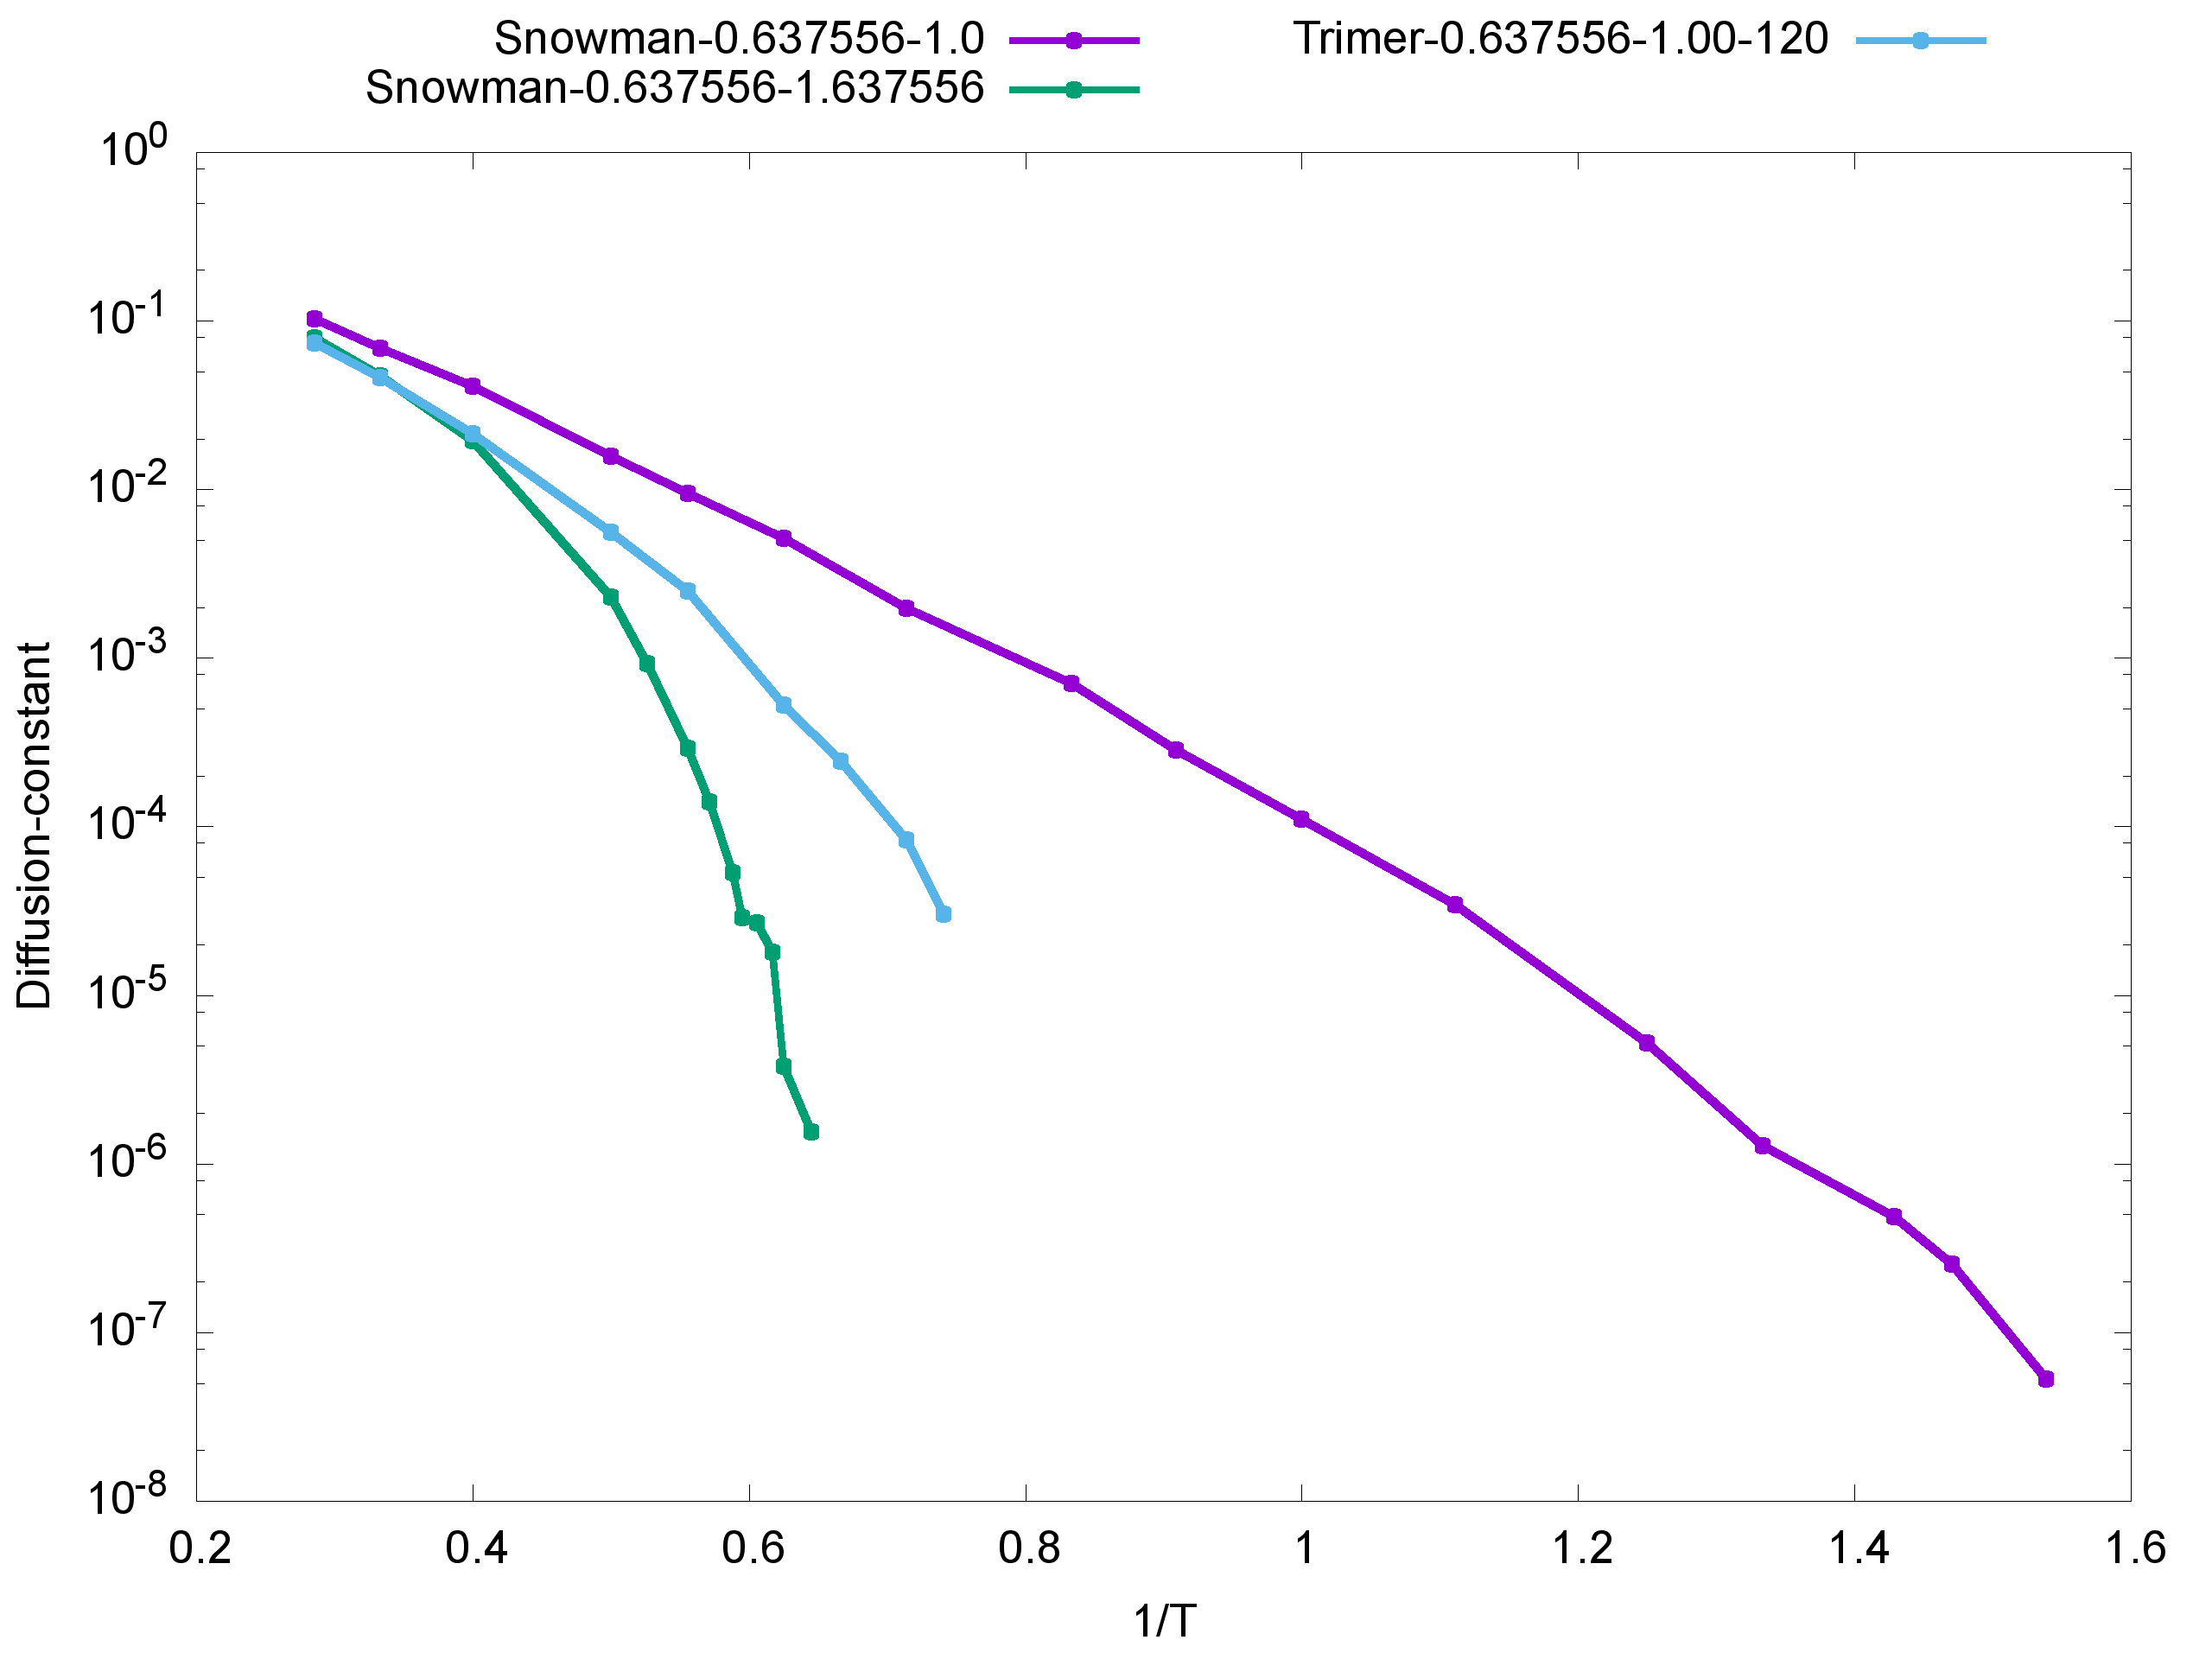
\includegraphics[width=\textwidth]{Diffusion-constant}
        \caption{Diffusion constant for all molecules}
        \label{fig:diffusion constant}
    \end{subfigure}
    \begin{subfigure}{0.5\linewidth}
        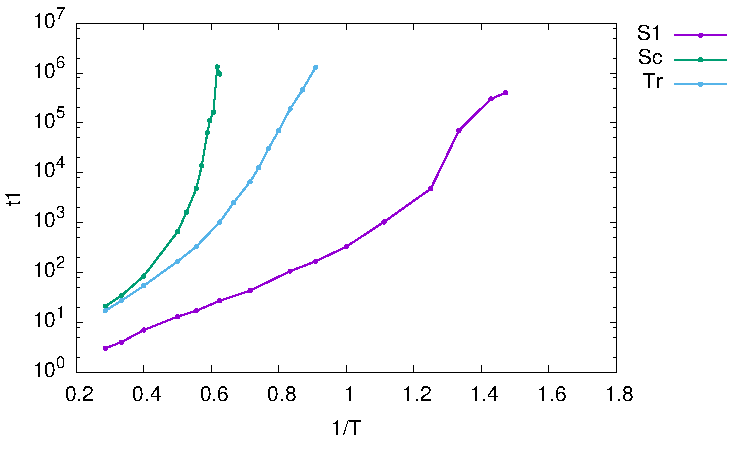
\includegraphics[width=\textwidth]{t1}
        \caption{Rotational relaxation time t1}
        \label{fig:tau1}
    \end{subfigure}
    \begin{subfigure}{0.5\textwidth}
        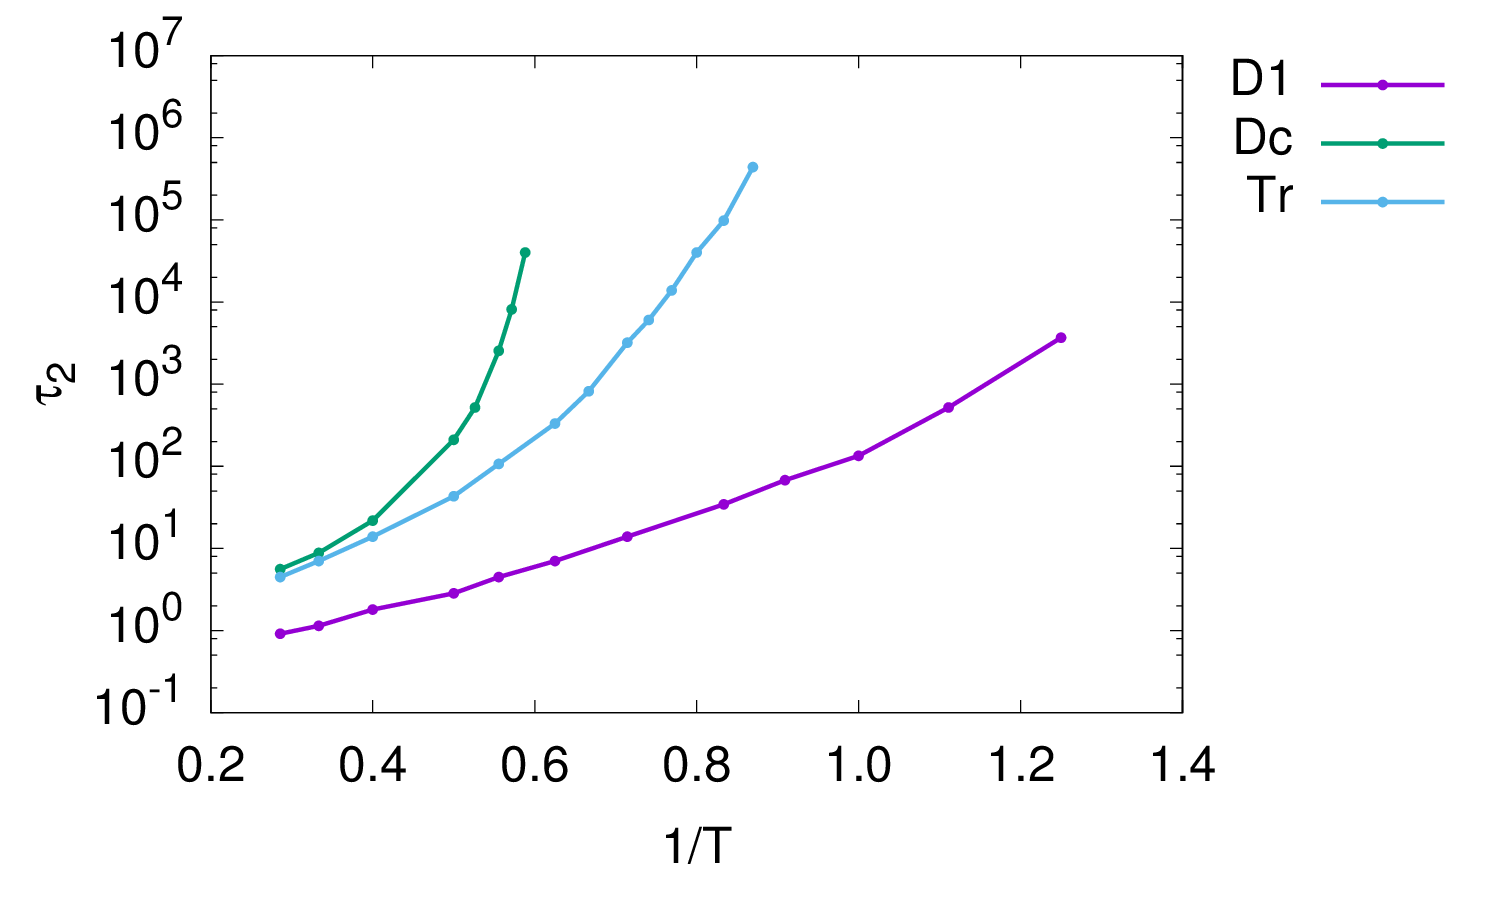
\includegraphics[width=\textwidth]{t2}
        \caption{Rotational relaxation time t2}
        \label{fig:tau2}
    \end{subfigure}
    \begin{subfigure}{0.5\textwidth}
        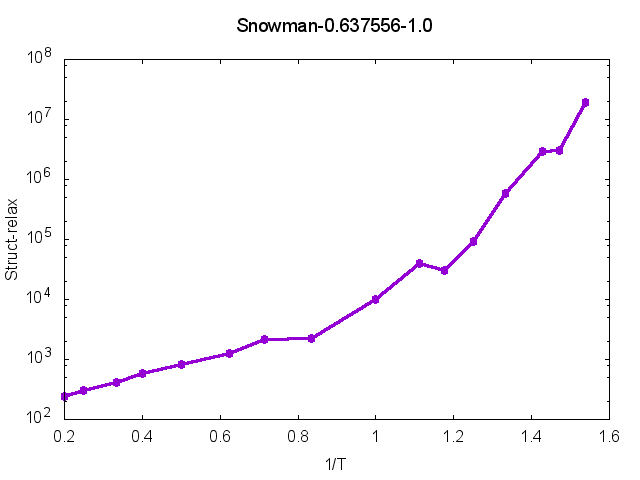
\includegraphics[width=\textwidth]{struct-relax}
        \caption{Structural relaxation times}
        \label{fig:struct relax}
    \end{subfigure}
    \caption{Comparison of dynamics quantities}
    \label{fig:dynamic comparison}
\end{figure}

From \textfigref{diffusion constant} we can see that as the size of the concavity increases from \sone, through \scon to \tri the fragility increases. This suggests that molecular shape is one of the features responsible for the fragility and by extension the formation of the glassy phase.
